\chapter{INTRODUCTION} 
\label{ch:intro}

In a broad sense, this dissertation explores the development of reinforcement learning based techniques suited to applications in nonlinear filtering (or nonlinear state estimation) and Markov chain Monte Carlo (MCMC) algorithms. During the initial development of this dissertation, a special class of approximate nonlinear filters called the feedback particle filter (FPF) was the primary focus. Later, by lucky coincidence, it was observed that similar techniques could be applied to obtain interesting results in MCMC algorithms as well. Hence, the chapter on MCMC forms a smaller portion of the dissertation. 

The goal of this chapter is a cursory introduction of the elements that are key to the problems considered in this dissertation. In \Section{s:goals}, we describe the two major goals undertaken - in the areas of nonlinear filtering and MCMC. Subsequently, in \Section{s:tools}, we introduce the various tools used, motivate the solution approaches adopted, without delving much into the technical details. 
\section{Goals of the Dissertation}
\label{s:goals}
\subsection{Nonlinear filtering/state estimation}
\label{s:filtering}
Consider a dynamic system evolving in time according to a given mathematical model. A complete characterization of the system is given by its states. Uncertainties in the system model or external disturbances are modeled as process noise, and indirect observations of the state, corrupted by measurement noise are available. The observation model and the noise statistics are assumed to be known. The state dynamics and observations may be in either continuous or discrete time depending on the system properties. The state dynamics are assumed to be Markovian, i.e. in rough terms, the probability of the current state just depends on the previous state, and not on the entire history. 

A generic block diagram of a state estimator is depicted in \Fig{Fig:state_estimator}. The goal of any filtering/state estimation problem is to recursively estimate the states of the system based on noisy partial observations. The top row of the block diagram, with the state and observation models, indicates the actual evolution of the system. The prediction and correction blocks form part of the state estimator. Given the current estimate of the state, the prediction block gives the best state estimate, called the prior estimate for the next time instant using the state model. The correction block updates the prior after receiving the most recent observation, and outputs the posterior estimate. All filtering approaches share this basic structure, although in some cases, the prediction and correction steps may be combined.  

\begin{figure}
	\centering
	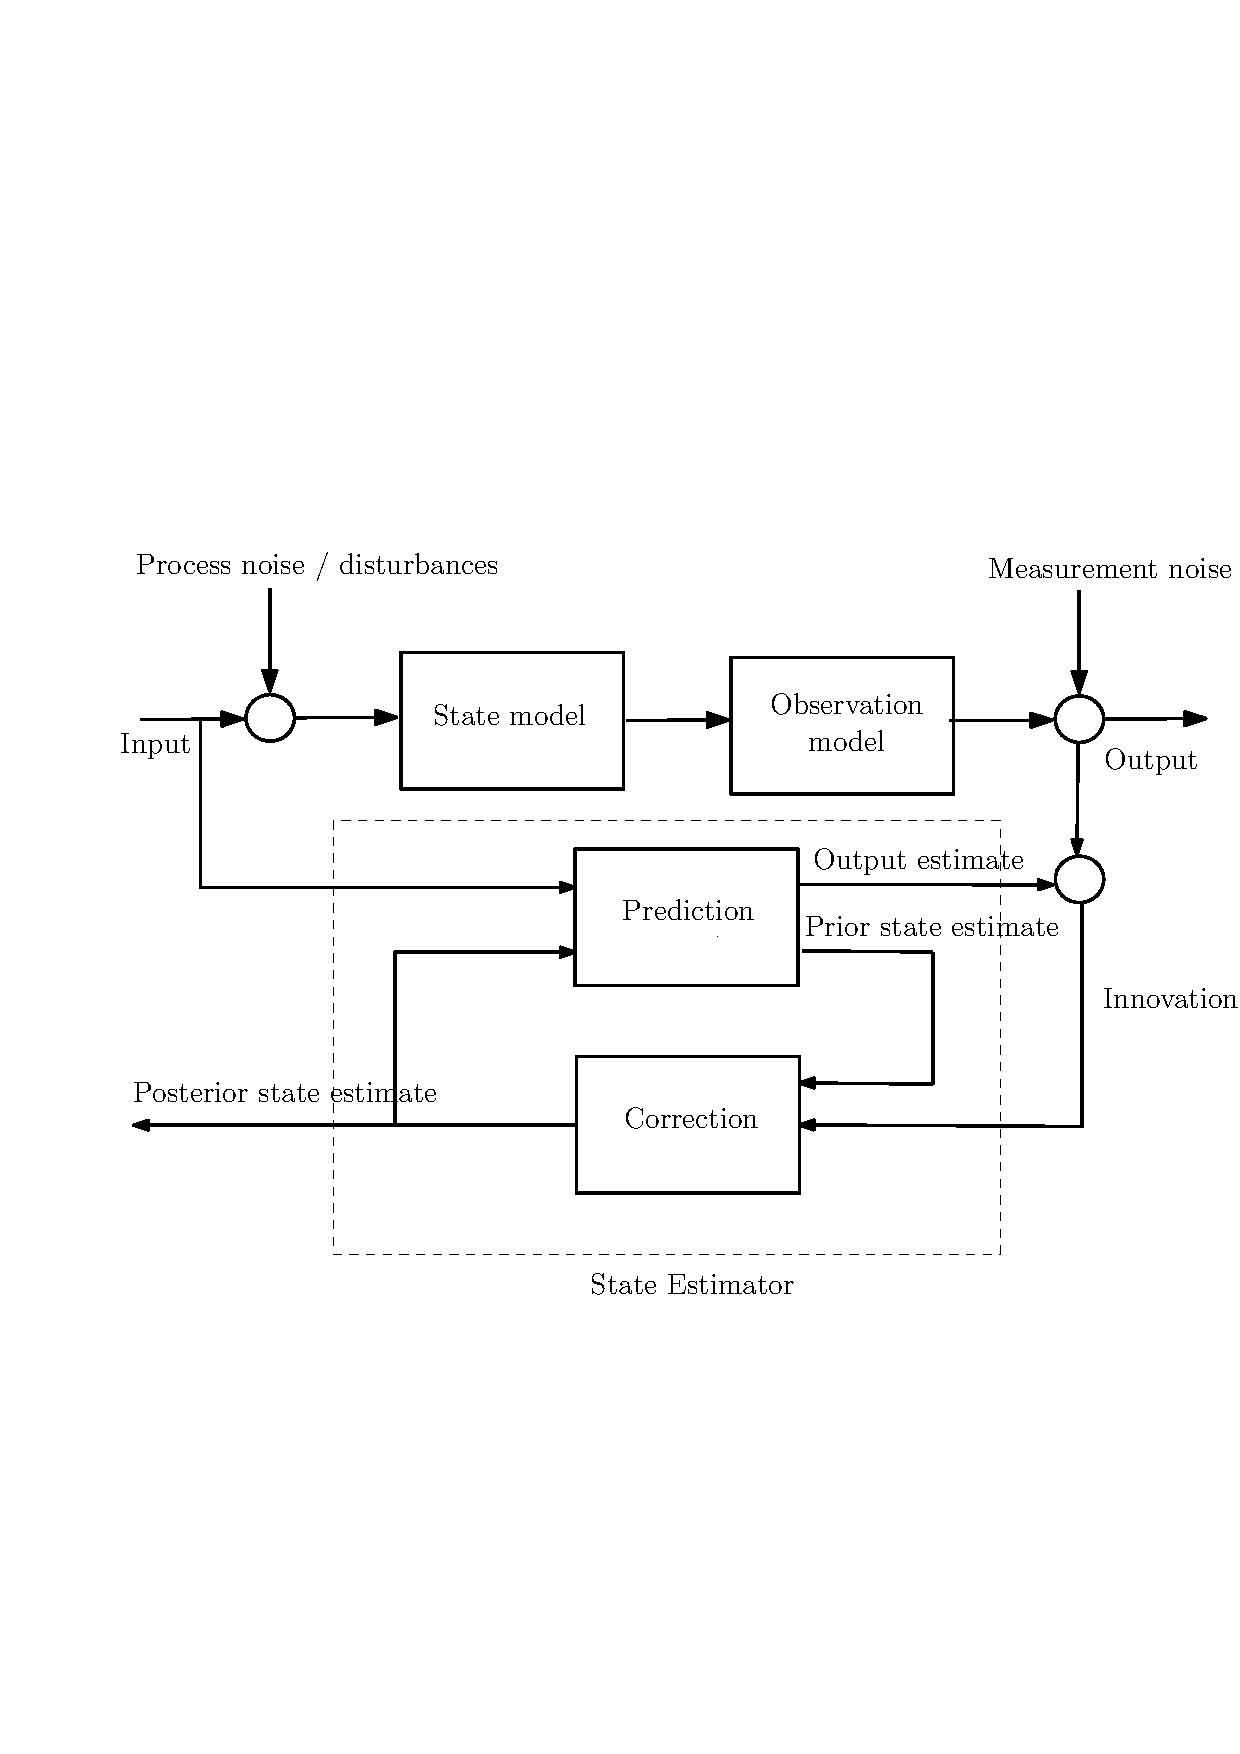
\includegraphics[width=7in]{images/Chap1_state_est_block}
	\caption{Block diagram of a state estimator}
	\label{Fig:state_estimator}
\end{figure} 
\anand{Need to verify if the block diagram is correct}
Initial applications of filtering included satellite orbit determination, aircraft navigation and tracking \cite{kutsurpfi19}. More recently, filtering has found applications in diverse areas such as machine learning \cite{bishop06}, queueing networks, mathematical finance \cite{brihan08} and data assimilation problems for weather forecasting \cite{eve94}. \anand{A simple example may be good here.}

When the system dynamics are linear and the noise quantities are Gaussian, the problem is simpler and the well-known Kalman filter is the optimal solution. The Kalman filter gives a linear SDE (stochastic differential equation) for the conditional mean of the state and a Riccati type ODE for the state covariance. These two quantities However, in practice, the linear state dynamics - Gaussian disturbances assumption is often violated.  For example, in weather forecasting the states evolve via a complex system of fluid mechanics equations that are nonlinear. The optimal solution is given by a set of SDEs, like the Zakai's equation or the Kushner-Stratonovich equation. The posterior estimates are in the form of conditional distributions of the state, given the entire history of observations. A detailed discussion of the nonlinear filtering theory can be found in \cite{baicri08}. 

Linear approximations like the extended Kalman filter (EKF) were studied for application to nonlinear systems. They perform well as long as the state or observation dynamics do not deviate significantly from linearity. Later with the advent of modern computing, Monte Carlo based methods like the conventional bootstrap particle filter gained popularity. The underlying principle here is to approximate the posterior distribution using empirical samples called particles. Budhiraja et al. \cite{budchelee07} provide a comprehensive survey of numerical methods for nonlinear filtering problems. 

The main focus of this dissertation is a class of controlled particle system algorithms called the feedback particle filter (FPF). Feedback particle filter was originally formulated for the continuous-time nonlinear filtering problem in the Euclidean setting \cite{yanmehmey13}. They have since been extended to Riemannian manifolds and matrix Lie groups \cite{zhatagmeh16}. The FPF is similar in its feedback structure to the Kalman filter and in its empirical approximation approach to the standard particle filter. In other respects, they are significantly different. A crucial component of the FPF is the gain function, which is analogous to the Kalman gain in the Kalman filter. The optimal gain function in the FPF is obtained as the gradient of the solution to a particular version of Poisson's equation \cite{yanmehmey13, laumehmeyrag14}. Obtaining an analytical solution to the Poisson's equation is often difficult and hence, approximation is required. In this dissertation, our main focus is on developing algorithms to approximate the gain function. A detailed discussion is reserved for \Chapter{ch:filtering}. 

\subsection{Markov chain Monte Carlo (MCMC) algorithms}
\label{s:mcmc}
The second application of interest is Markov chain Monte Carlo (MCMC) algorithms. MCMC algorithms have a long history of being applied to problems in Bayesian statistics \cite{}. \anand{citation needed}

In standard Monte Carlo methods, expectation of a function $f$ of a random variable $X$ distributed according to a density $\pr$ is approximated empirically as,
\begin{equation}
 \Expect_{X \sim \pr} [f(X)] \eqdef \int_\state f(x)\pr(x) dx \approx \frac{1}{N} \sum_{i=1}^N f(X_i)
 \label{e:intro_emp_avg} 
\end{equation}
where each $X_i$ is distributed according to $\pr$ and $N$ is sufficiently large. As is often the case, it may be difficult to generate a sequence of samples $\{X_i\}_1^N$ according to the desired target distribution $\pr$. Methodologies such as rejection sampling and importance sampling make use of an easy-to-sample surrogate distribution to sample from the original target distribution. But, if $\pr$ is high-dimensional, it is difficult to find a closely matching simple surrogate distribution. 

MCMC algorithms provide an alternative solution in this situation. They are a special class of Monte Carlo methods in which the samples $X_i$ are the states of an ergodic Markov chain. Given the target density $\pr$, the problem reduces to finding an appropriate transition kernel for a Markov chain that has $\pr$ as its invariant density. The Langevin diffusion, which is a perturbed gradient flow with respect to a potential function in continuous time, forms the basis of many such algorithms. The Gibbs algorithm \cite{tanwon87} and Metropolis-Hastings (M-H)  algorithm \cite{has70} are popular discrete-time MCMC techniques. They have been widely applied for problems in Bayesian inference, statistical physics, computation biology etc.

%MCMC algorithms are a popular means of sampling from high dimensional densities. Typically, computing expectations of functions via integration is infeasible in high dimensions and MCMC algorithms provide a method to obtain numerical approximations to the expectation. 
The asymptotic convergence of the empirical averages of the form \eqref{e:intro_emp_avg} to the true expected value is guaranteed under general conditions by law of large numbers. The main drawback of these techniques as compared to standard Monte Carlo sampling which provides independent and identically distributed (i.i.d.) samples, is that the successive samples of the Markov chain are correlated to each other. This results is slower convergence of the algorithms. The central limit theorem states that,
\begin{equation}
\sqrt{N} \Bigl(\frac{1}{N} \sum_{i=1}^N f(X_i) - \Expect_{X \sim \pr} [f(X)] \Bigr) \overset{d}{\to} \normal(0, \asymvar^2),\qquad \text{as } N \to \infty, 
\end{equation}
where $\mathcal{N}(0,1)$ refers to the standard Gaussian distribution with mean zero and unit variance. Asymptotic variance $\asymvar^2$ is a measure quantifying the rate of convergence. Lower its value, faster is the convergence of the Markov chain to its invariant distribution and hence, the goal is to minimize it. 

Asymptotic variance can be expressed in terms of the solution to Poisson's equation \cite{ctcn}. Control variates, which are zero-mean terms added to the function $f$, have been used to reduce the asymptotic variance of the estimates without adding any bias. Henderson, in his dissertation \cite{henthesis97} notes that the best choice of control variates can be constructed using the solution to Poisson's equation. They also feature prominently in Chapter 11 of the book \cite{ctcn} with the objective of constructing reduced-variance estimators for network models. Control variates constructed using the fluid value function have been shown to produce a $100$-fold reduction in variance over the standard estimator for the KSRS queueing model in the examples considered in the book chapter. 

In this dissertation, we demonstrate that the same algorithms we propose for approximating the FPF gain function, find additional application in improving the performance of popular MCMC algorithms. 
% Section 11.2.1 and Section A.5 of CTCN, 
% Control variates - Prop 8.2.4 and Theorem A.5.4

\section{Tools Used in the Dissertation}
\label{s:tools}
Now, that the main application areas of the dissertation have been described briefly, we introduce the various tools that help us achieve our goal. In \Section{s:poissons}, a preliminary description of the Poisson's equation, that is crucial to both our applications of interest is given.
\subsection{Poisson's equation} 
\label{s:poissons}
In its most general form, Poisson's equation is a second-order differential equation of the form,
\begin{equation*}
\generate h \eqdef - f,
\end{equation*}
where $\generate$ is a second-order differential operator. Usually, $f \in C^2$ is given and is ``centered'' by subtracting its mean. The function $h$ is unknown and is called the solution to the Poisson's equation. In Physics, the operator $\generate$ is often taken to be the Laplacian. Poisson's equation appears widely in the context of Markov chains and stochastic optimal control. In the context of a continuous-time diffusion process, the operator $\generate$ refers to the infinitesimal generator, also called the differential generator.  \anand{ If $f \equiv 0$, then $h$ is precisely harmonic functions \cite{glymey96a}}.

Poisson's equation is central to average-cost optimal control theory. In this case, $f$ is a one-step cost function and $h$ is called a relative value function. \anand{The states evolve in the form of a controlled Markov chain based on a given policy.} Relative value function gives the infinite-horizon expected cost when starting from a given state under this stationary policy. Approximate solutions to the equation lead to direct performance bounds of the control algorithm \cite{ctcn}. Explicit bounds on the solution $h$ have been obtained under general conditions of the chain in \cite{}. \anand{citation needed}
% measure of long-term system performance in \cite{brabar96}.

Our interest lies in a particular version of Poisson's equation associated to the Langevin diffusion process. Langevin diffusion is discussed in greater detail in \Section{s:langevin_diffusion} and \Section{s:langevin_mcmc}. Gradient of the solution to this equation is the optimal choice of the gain function associated with the FPF \cite{yanmehmey13}. In MCMC algorithms, as noted by Henderson \cite{henthesis97} and later by Dellaportas et al. \cite{delkon12}, the optimal control variates can be constructed from this solution. Thus, Poisson's equation and its solution are central to the goals of this dissertation. 

Obtaining a closed form solution is difficult outside of special cases and this motivates the study of approximation algorithms. Various approaches have been studied such as the Markov semigroup approximation by Taghvaei et al. \cite{tagmeh16a}. Finding an approximate solution falls within the framework of reinforcement learning and in particular, temporal difference (TD) learning. In this dissertation, we develop variants of the TD learning algorithm that can approximate the gradient of the solution to Poisson's equation directly.

% basis for much of ergodic theory of Markov chains \cite{ctcn}


\subsection{Reinforcement learning and TD learning}
\label{s:rl_td}
In this section, a beginner level introduction to reinforcement learning algorithms is provided. Reinforcement learning algorithms have gained popularity over the last decade having achieved major successes in a wide variety of applications like AlphaGo, backgammon etc. \anand{need references} In a general setting, such algorithms involve learning what actions to take in a given situation, so as to maximize a numerical reward (or equivalently minimize a numerical cost) over a (possibly infinite) time-horizon. The learned set of actions, called a policy is a mapping from the state space to the action space. In a stochastic setting, this mapping is expressed in terms of probability of taking a particular action in a given state. The learning is performed purely based on interactions with the environment without any prior knowledge of the system model. A whole variety of algorithms including Q-learning \cite{watday92a} and temporal difference (TD) learning \cite{sut88} belong to this category. A slightly different class of algorithms that makes use of model information also exists, called approximate dynamic programming. \anand{needs rephrasing}
Although, the end objective is to obtain optimal policies, a central theme in all these algorithms is value function approximation. This aspect is what makes these algorithms an attractive choice for our objective. 

Sutton and Barto write in their monograph \cite{sutbar98}, ``If one had to identify one idea as central and novel to reinforcement learning, it would undoubtedly be temporal difference learning''. Originally introduced by Sutton in \cite{sut88}, TD learning algorithms address the problem of policy evaluation associated with discrete-time stochastic optimal control problems called Markov decision processes (MDPs). In other words, for a given fixed policy, the algorithm computes estimates of the value function through an iterative procedure. A large body of prior research is available that studies the asymptotic convergence properties of these algorithms. Most of them, however are restricted to either the discounted-cost case or an undiscounted-cost (average-cost) setting for a finite state space Markov chain with an absorbing state. Both these assumptions are violated in the context of approximating the solution to Poisson's equation of interest to us. Hence, the need to develop new algorithms. 

A least-squares approach to TD learning, introduced by Bradtke et al. \cite{brabar96},  has been discussed in the context of value function estimation for a fixed policy in \cite{ctcn}. An appropriate learning objective is chosen based on the context. For example, in optimal control, the goal is to optimize performance over the class of policies, whereas in MCMC, minimizing the asymptotic variance is the chosen criterion. Least squares TD (LSTD) learning aims to obtain approximations to the true value function from within a parameterized family of functions. The learning problem is thus reduced to finding the best approximation based on a chosen criterion from within this class. Section 11.5.2 of \cite{ctcn} presents the LSTD learning algorithm for the discounted-cost problem. Recursive update rules are presented for the parameter weights and they have been shown to converge asymptotically to the optimal values. In Section 11.5.4, the results are generalized to the average-cost setting, which requires solving the Poisson's equation. However, the application of LSTD algorithm in this case is justified only if a regenerating state for the Markov chain exists. This rules out its application to state spaces in higher dimensions.

In this dissertation, we follow the key ideas presented in Section 11.5.2 to develop a new class of algorithms called differential LSTD learning that approximates the gradient of the solution to Poisson's equation directly.  The algorithm design enables the construction of a Monte Carlo based technique that scales well in high dimensions. This is achieved by introducing an implicit discounting factor, that ensures the existence of a regenerating state for the process. For the special case of Langevin diffusion, using the self-adjoint property of the differential generator, we obtain a simple and elegant version of the algorithm in \Section{s:diff_td_langevin}.  A more general version of the algorithm that can be applied to any continuous-time diffusion processes is presented in \Section{s:diff_td_learning}. 
A similar algorithm for discrete-time examples with applications to optimal control is presented by Devraj et al \cite{devmey16arXiv}.
 
% nonlinear parameterization in Section 11.5.3 
% average-cost TD learning based on \cite{kontsi03a}
\subsection{Reproducing kernel Hilbert space (RKHS)}
\label{s:rkhs}
Traditionally, TD learning has been tested on spaces spanned by a carefully chosen finite set of basis functions. However, there are no standard approaches to choosing the basis.  If any insight about the structure of the true value function is available, this can be exploited in choosing an appropriate function class. In optimal control problems, this insight is available in the form of fluid value functions. But this is not true for Poisson's equation of interest. One of the novelties of this dissertation is the use of reproducing kernel Hilbert space (RKHS) as an approximating function space for TD learning algorithms. This simplifies the choice of problem dependent basis functions by making use of the information about particle locations effectively. 
 
Reproducing kernel Hilbert spaces form an important class of function spaces in learning theory \cite{aro50, schsmo01}. They are complete Hilbert spaces uniquely characterized by a kernel function. The use of RKHS for function approximation provides us with greater flexibility and potentially a richer function class. Although optimization in an RKHS is typically infinite dimensional, they are endowed with useful properties that help us reduce the problem to finding a finite set of parameters via the representer theorem \cite{kimwah71, schhersmo01}. A brief background of the RKHS theory along with properties that make them useful in this dissertation is provided in \Chapter{ch:rkhs}. The differential TD learning algorithm specific to the Langevin diffusion is adapted to accommodate an RKHS as the approximating function space in \Chapter{ch:rkhs}.
 

\section{Dissertation Outline}
\label{s:outline}
The various topics discussed in this chapter may seem distinct and disconnected. This dissertation attempts to tie them together as it progresses. To summarize, we restrict our attention to approximating solutions of a particular version of the Poisson's equation. Differential TD learning algorithms using a finitely parameterized family of functions and an RKHS are studied and presented. Approximations obtained using these algorithms are tested and have been shown to improve the performance of the FPF and MCMC algorithms. 

The main contributions of this dissertation that form the remaining chapters can be summarized as - i) development of differential LSTD learning algorithm, similar to LSTD in \cite{ctcn} to approximate the gradient of the solution to Poisson's equation directly in \Chapter{ch:diff_td}, ii) refinement of this algorithm with a simpler resolution \cite{radmey18a} in \Section{s:diff_td_langevin}, iii) address the problem of basis selection by the use of RKHS in Chapter \ref{ch:rkhs}, iv) applications to nonlinear filtering in \Chapter{ch:filtering} and MCMC algorithms in \Chapter{ch:mcmc}. Finally, conclusions and scope for future work are included in Chapter 6.  

\section{Notation}
\label{s:notation}
$\bfmX\eqdef \{X_t: t\ge 0\}$ is a stochastic process, evolving on the state space  $\state$, which is taken to be $\Re^d$, unless specified. A subscript notation $X_t$ is often used to denote $X(t)$, where $t$ is an index of time. The symbol $\pr$   denotes a probability density on $\state$, and $L^2(\state,\pr)$ is the Hilbert space of square integrable functions with the usual inner product,
$\langle \phi,\psi\big\rangle_{L^2}\eqdef\int\phi(x)\psi(x) \pr(x)\ud x$, where $\phi$ and $\psi$ are scalar valued functions in $L^2(\state, \pr)$;
written $L^2$ when there is no risk of ambiguity.  The associated norm is
denoted   $\|\phi\|^2_{L^2}\eqdef\langle\phi,\phi\rangle_{L^2}$. The inner product is extended to vector valued functions $f,g: \state \to \Re^d$ by defining, $\langle f, g \rangle_{L^2} \eqdef \sum_{k=1}^d \langle f_k, g_k \rangle_{L^2}$. The expectation of a function $f$ with respect to $\pr$ is written as $\Expect_{X \sim \pr}[f(X)]$ and the  notation $\Expect_x$ is used as shorthand for the conditional expectation $\Expect_x[f(X_t)] \eqdef \Expect[f(X_t)|X_0 = x]$.  We use $\|\cdot\|$ without the subscript to refer to the Euclidean norm and $\|\cdot \|_\infty$ refers to the maximum or uniform norm. 

Another Hilbert space $\clH$ will appear in the application of reproducing kernel Hilbert space theory with its inner product denoted   $\langle \varble, \varble \rangle_{\clH}$,  and induced norm    $\| \varble \|_\clH$. $C^k$ is used to denote the space of $k$-times continuously differentiable functions $f\colon\state\to\Re$,
$\nabla f $ denotes the gradient of a function $f\in C^1$, and $\Delta f$ the Laplacian for $f\in C^2$. If $\state = \Re$, the notation $f'$ and $f''$ are often used to denote the first and second derivatives respectively.

%The remainder of the dissertation is organized as below. In Chapter \cite{}, we discuss the problem set up, i.e. the Poisson's equation for Langevin diffusions and introduce differential TD learning} to obtain approximate solutions. A simpler resolution to the problem is proposed and an algorithm derived using this resolution is presented in Chapter \cite{}. In Chapter \cite{}, we discuss the application to nonlinear filtering in detail along with some numerical results. The second application to MCMC algorithms is presented with numerical examples in Chapter \cite{}. Finally, we present conclusions and scope for future work in Chapter \cite{}. 
 


 

%\begin{figure}[htbp]
%  \centering
%    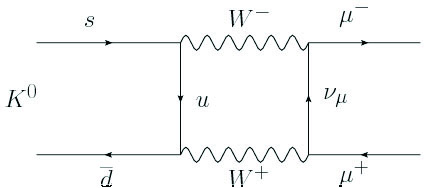
\includegraphics[width=5in]{images/diagram}
%    \caption[EPS format diagram. Note: no filetype is designated by adding an extension.]{EPS format diagram. Note: no filetype is designated by adding an extension. The file type is determined and the correct procedure is automatically chosen by xelatex.}
%\end{figure}
%
%
%
%\begin{figure}[htbp]
%     \centering
%   \mbox{
%      \subfigure [] {
\includegraphics[scale=0.6]{images/mouse}} \qquad
%      \subfigure []{
\includegraphics[scale=0.6]{images/mouse}} \qquad
%     }
%    \mbox{
%      \subfigure [] {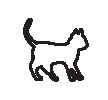
\includegraphics[scale=3]{images/cat}} \qquad
%      \subfigure [] {
\includegraphics[scale=0.6]{images/mouse}} \qquad
%      }
%    \caption[Tom and Jerry]{Tom and Jerries. This caption demonstrates how the sub-captions are left out of the List of Figures, but included in the figure itself. A) Tom the first; B) Tom the second; C) Jerry; D) Tom the third.}
%    \label{mice}
%  \end{figure}

